\documentclass{article}

\usepackage{pgfplots}

\pgfplotsset{compat=1.13}

% \usetikzlibrary{}
\usepgfplotslibrary{polar}

\usepackage{pgfplotstable}
\usepackage{booktabs}
\usepackage{array}
\usepackage{colortbl}

\begin{document}

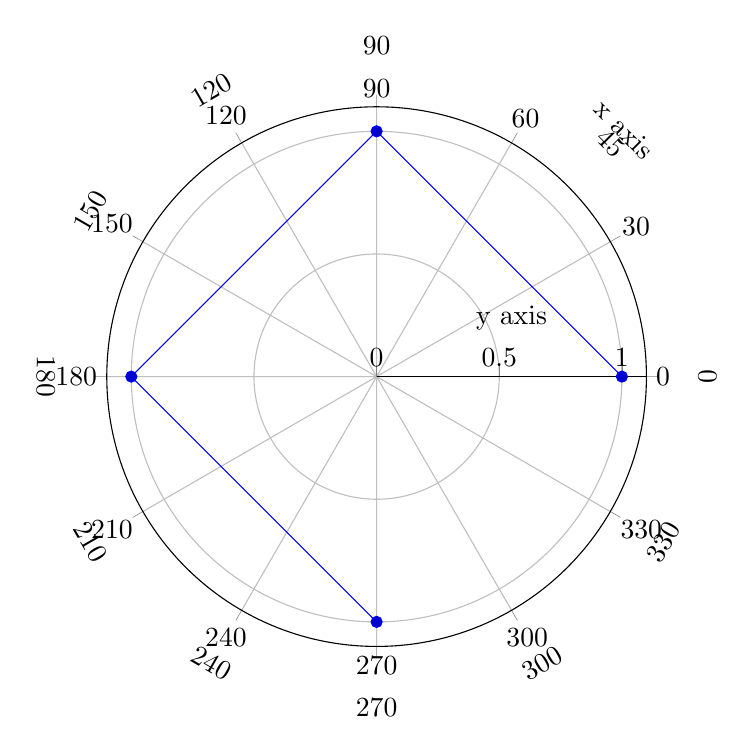
\begin{tikzpicture}
\begin{polaraxis}[
	xlabel=x axis,
	ylabel=y axis,
	extra description/.code={%
		\foreach \X in {0,45,90,120,150,180,210,240,270,300,330} {
			\pgfmathparse{\X/360}\let\XX=\pgfmathresult
			\node[sloped like x axis={at position=\X}]
				at (xticklabel cs:\XX) {\X};
		}
	},
]
\addplot coordinates {(0,1) (90,1)
	(180,1) (270,1)};
\end{polaraxis}
\end{tikzpicture}

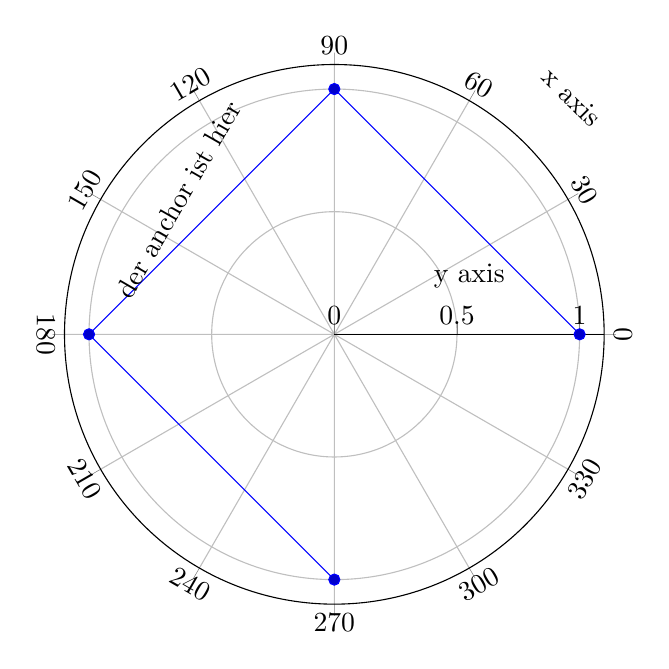
\begin{tikzpicture}
\begin{polaraxis}[
	xlabel=x axis,
	ylabel=y axis,
	xticklabel style={sloped like x axis},
	extra description/.code={%
		\node[anchor=near xticklabel, 
			sloped like x axis={at position=150}
		] 
			at (axis cs:150,1.1) {der anchor ist hier};
	},
]
\addplot coordinates {(0,1) (90,1)
	(180,1) (270,1)};
\end{polaraxis}
\end{tikzpicture}
\end{document}

